\documentclass[tikz,border=8pt]{standalone}
% Shared look for every TikZ diagram. Load with \input{../../tools/tikz-style.tex}
\usepackage[sfdefault]{roboto}
\usetikzlibrary{arrows.meta, positioning, shapes.geometric, calc, fit, backgrounds}
\definecolor{cblue}{HTML}{4C78A8}
\definecolor{corange}{HTML}{F58518}
\definecolor{cgreen}{HTML}{54A24B}
\definecolor{cred}{HTML}{E45756}
\definecolor{cpurple}{HTML}{B279A2}
\definecolor{cgrey}{HTML}{6B6B6B}
\tikzset{
  every picture/.style={font=\sffamily, line width=1.2pt},
  box/.style={draw=#1, fill=#1!12, rounded corners=4pt, align=center, inner sep=7pt, minimum height=1.1cm},
  box/.default=cgrey,
  arrow/.style={-{Stealth[length=3mm]}, draw=cgrey, line width=1.4pt},
  title/.style={font=\sffamily\bfseries\Large},
  note/.style={font=\sffamily\small, text=cgrey, align=center},
}
\AtBeginDocument{\hyphenpenalty=10000 \exhyphenpenalty=10000}

% Cascades in two open-source stacks, read from their code (paths in the Note's Sources).
% PX4 multicopter: position P -> velocity setpoint (capped) -> velocity PID -> acceleration -> attitude P -> rate setpoint
% (capped) -> rate PID with feedforward -> torque. Apollo longitudinal control: station PID -> speed offset -> speed PID
% -> acceleration, plus the planned acceleration (feedforward) and a slope term.
\begin{document}
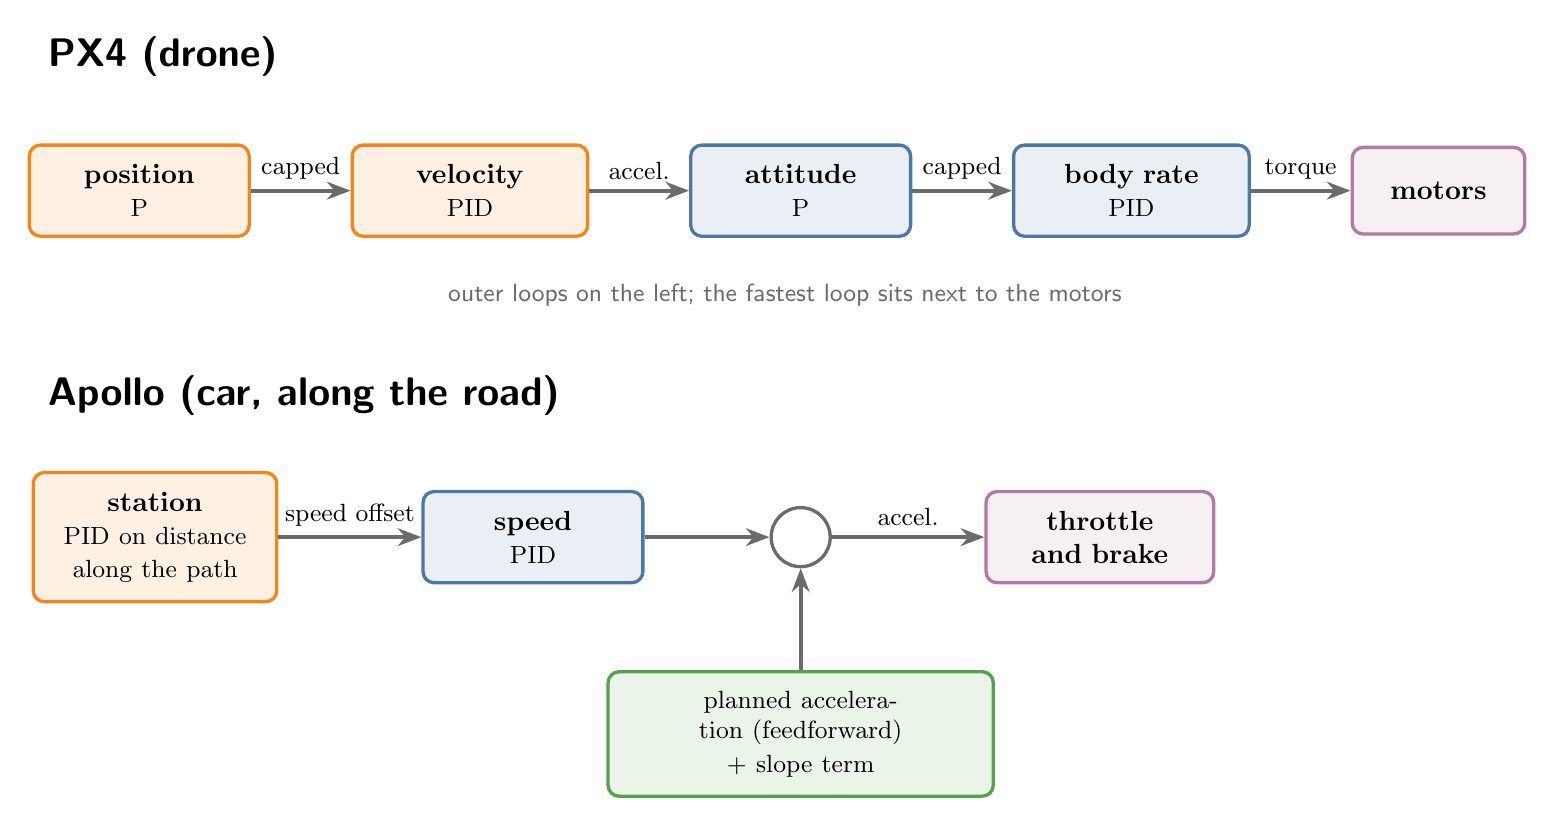
\begin{tikzpicture}[every node/.append style={font=\normalsize}]
  \node[title, anchor=west] at (-1.3,1.7) {PX4 (drone)};
  \node[box=corange, text width=2.3cm] (p1) at (0,0) {\textbf{position}\\ \small P};
  \node[box=corange, text width=2.5cm] (p2) at (4.2,0) {\textbf{velocity}\\ \small PID};
  \node[box=cblue, text width=2.3cm] (p3) at (8.4,0) {\textbf{attitude}\\ \small P};
  \node[box=cblue, text width=2.5cm] (p4) at (12.6,0) {\textbf{body rate}\\ \small PID};
  \node[box=cpurple, text width=1.7cm] (p5) at (16.5,0) {\textbf{motors}};
  \draw[arrow] (p1) -- node[above, font=\small] {capped} (p2);
  \draw[arrow] (p2) -- node[above, font=\small] {accel.} (p3);
  \draw[arrow] (p3) -- node[above, font=\small] {capped} (p4);
  \draw[arrow] (p4) -- node[above, font=\small] {torque} (p5);
  \node[note, anchor=north] at (8.2,-1.05) {outer loops on the left; the fastest loop sits next to the motors};
  \node[title, anchor=west] at (-1.3,-2.6) {Apollo (car, along the road)};
  \node[box=corange, text width=2.6cm] (a1) at (0.2,-4.4) {\textbf{station}\\ \small PID on distance along the path};
  \node[box=cblue, text width=2.3cm] (a2) at (5.0,-4.4) {\textbf{speed}\\ \small PID};
  \node[circle, draw=cgrey, fill=white, minimum size=0.75cm, inner sep=0pt] (a3) at (8.4,-4.4) {};
  \node[box=cgreen, text width=4.4cm] (aff) at (8.4,-6.9) {\small planned acceleration (feedforward)\\ + slope term};
  \node[box=cpurple, text width=2.4cm] (a4) at (12.2,-4.4) {\textbf{throttle and brake}};
  \draw[arrow] (a1) -- node[above, font=\small] {speed offset} (a2);
  \draw[arrow] (a2) -- (a3);
  \draw[arrow] (aff) -- (a3);
  \draw[arrow] (a3) -- node[above, font=\small] {accel.} (a4);
\end{tikzpicture}
\end{document}
